\section{DFiant HDL}
DFiant~\cite{Port2017} is a hardware description language (HDL) and one of the LEGaTO programming models. For a long time, the dominating HDLs have been Verilog, System Verilog, and VHDL, and they all provide the same register transfer-level (RTL) hardware design abstraction. An RTL language burdens designers with explicitly clocked constructs that do not distinguish between design functionality and implementation constraints (e.g., timing, target device).
For example, VHDL and Verilog constructs require designers to explicitly place a register, regardless if it is part of the core functionality (e.g., a state-machine state register), an artifact of the timing constraints (e.g, a pipeline register), or an artifact of the target interface (e.g., a synchronous protocol cycle delay). These semantics narrow design correctness to specific timing restrictions, while vendor library component instances couple the design to a given target device. Evidently, formulating complex portable designs is difficult, if not impossible. Finally, these older languages do not support modern programming features that enhance productivity and correctness such as polymorphism and type safety.

High-level synthesis (HLS) tools such as Vivado HLS~\cite{Vivado2012}, and high-level HDLs such as Bluespec SystemVerilog~\cite{nikhil2004bluespec} and Chisel~\cite{Bachrach2012} attempt to bridge the programmability gap.
While these tools and languages tend to incorporate modern programming features, they still mix functionality with timing and device constraints, or lack hardware construction and timed synchronization control. On one hand, Chisel and Bluespec constructs explicitly pipeline designs. And on the other hand, Vivado HLS C++ constructs cannot directly support a simple task as toggling a led at a given rate.
Such tools and languages, therefore, fail to deliver a clean separation between functionality and implementation that can yield portable code, while providing general purpose HDL constructs. 

\begin{figure}[h]

\centering

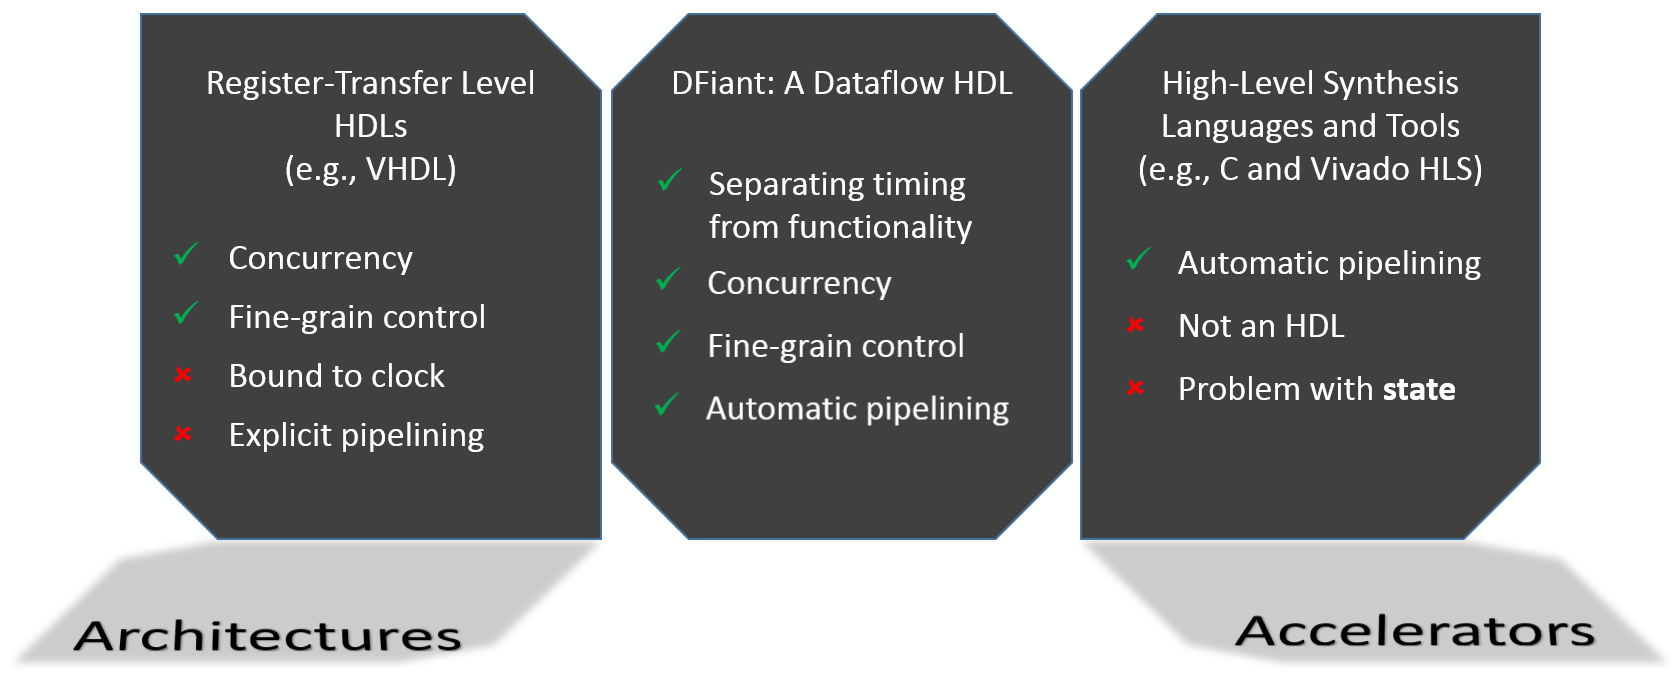
\includegraphics[scale=0.2]{graphics/dfiant_prog_gaps.png} 

\captionof{figure}{DFiant fills in the programmability gaps}

\label{fig:prog_gaps}

\end{figure}

Figure \ref{fig:prog_gaps} summarizes the primary programmability pros and cons of RTL and HLS languages with their targeted programming domains, architectures and accelerators, respectively. DFiant aims to bridge over the programmability gaps by combining constructs and semantics from software, hardware and dataflow languages. DFiant is \emph{not} an RTL language, nor is it a sequential HLS language such as C. Instead, the DFiant programming model accommodates a middle-ground approach between low-level hardware description and high-level sequential programming.   

DFiant is a modern HDL whose goal is to improve hardware programmability and designer productivity by enabling designers to express truly portable and composable hardware designs.
DFiant decouples functionality from timing constraints (in an effort to end the \emph{"tyranny of the clock"}~\cite{Sutherland2012}). DFiant offers a clean model for hardware construction based on its core characteristics:
\begin{enumerate*}[label=(\roman*)]
\item
  a clock-agnostic dataflow model that enables implicit parallel data and computation scheduling; and
\item
  functional register/state constructs accompanied by an automatic pipelining process, which eliminate all explicit register placements along with their direct clock dependency.
\end{enumerate*}   

DFiant is implemented as a Scala library and relies on Scala's strong, extensible, and polymorphic type system to provide its own hardware-focused type system (e.g., bit-accurate dataflow types, input/output port types). The library performs two main tasks: the frontend compilation, which translates dataflow variable interactions into a dependency graph; and the backend compilation, which translates the graph into a pipelined RTL code and a TCL constraints file, followed by a hardware synthesis process using commercial tools. DFiant can be used in any Scala-compatible IDE, including the LEGaTO eclipse-based tool-chain.



